\section{Business Model Canvas}
Durch die Erkenntnisse der vorherigen Konzepte erstellt das Agrishare-Team ein \ac{BMC}, welches in Abschnitt \ref{BMC_Kapitel} genauer erklärt wird. Ein erster Entwurf der Canvas ist in Abb. \ref{BMC_Agrishare} dargestellt.
\begin{figure}[h!]
		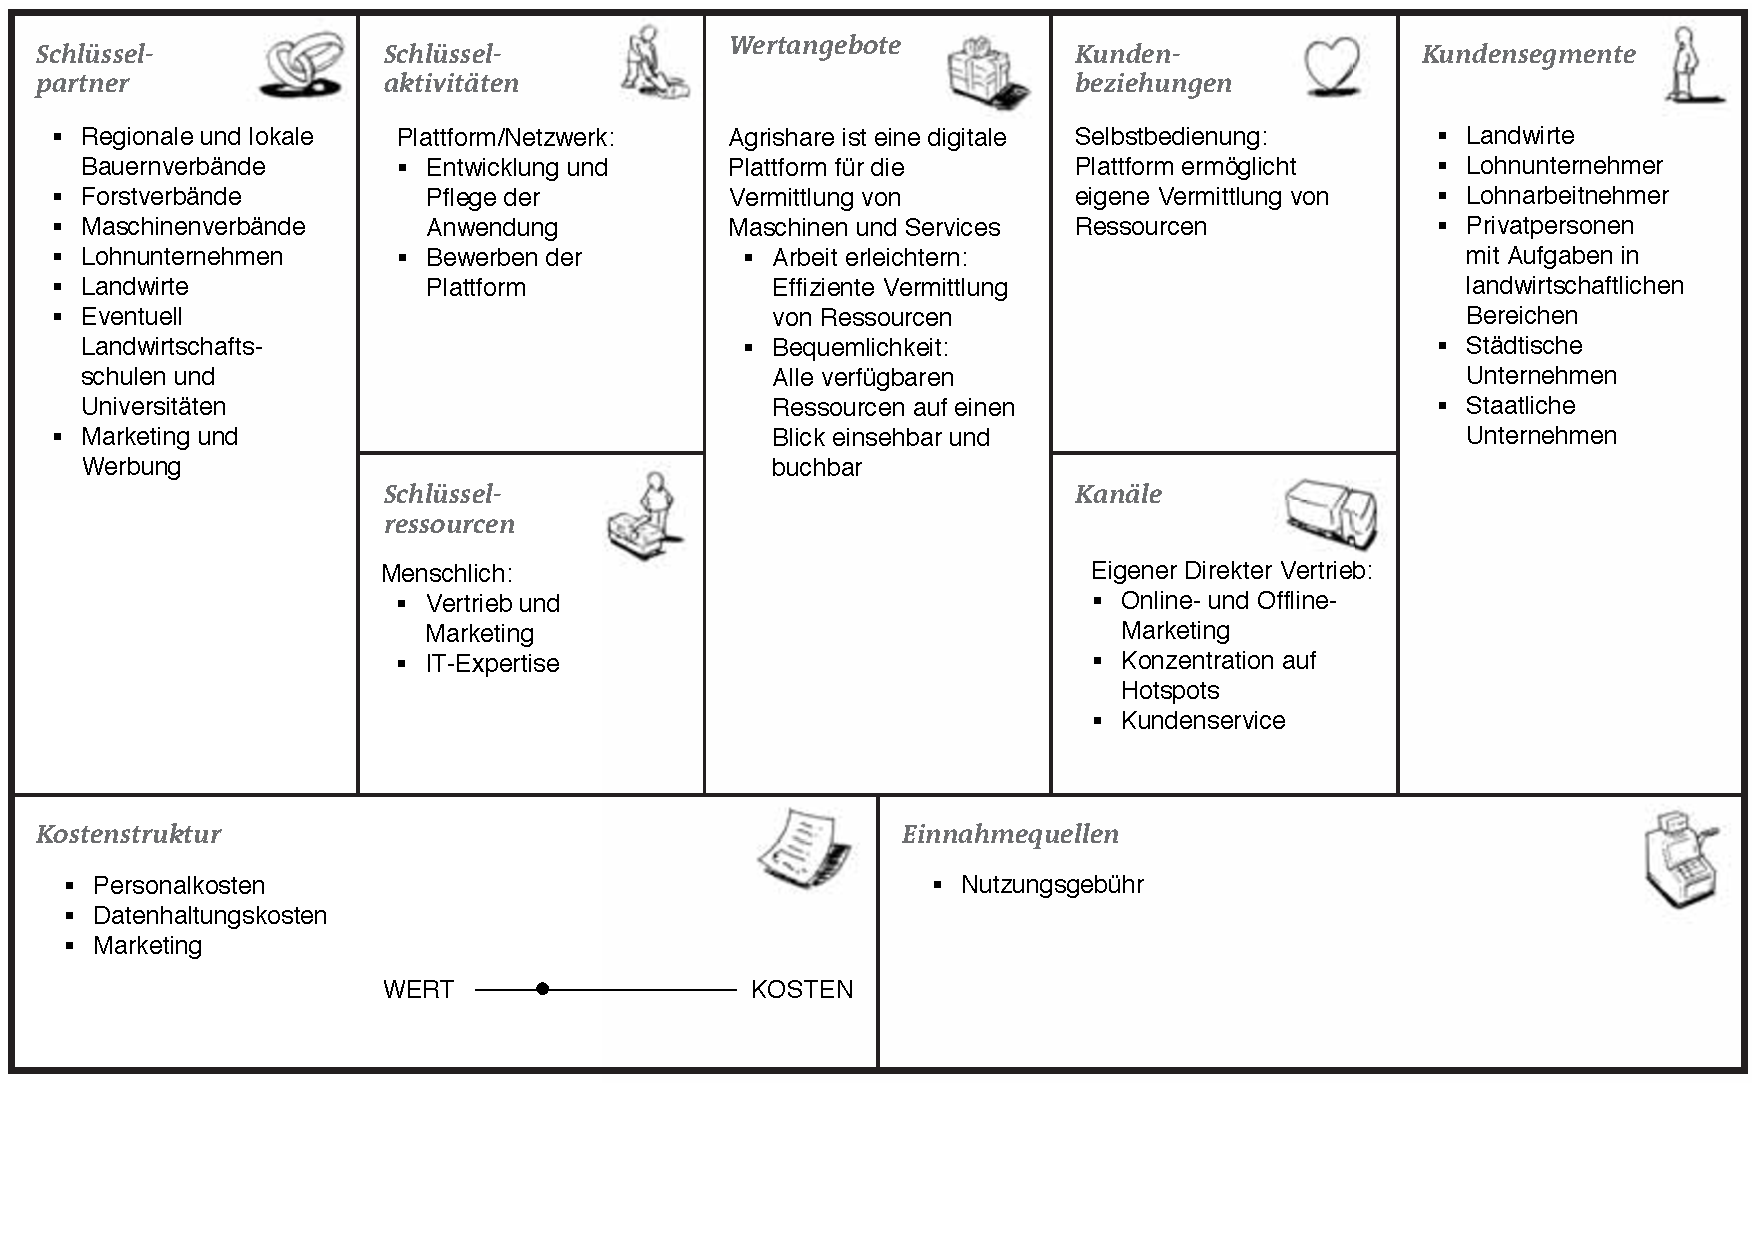
\includegraphics[angle=90,origin=c,width=\textwidth]{99_PDF_INCLUDE/BMC_draft.pdf}
		\caption{\ac{BMC} Agrishare}
		\label{BMC_Agrishare}
\end{figure}

Das Kundensegment ist hier als Nischenmarkt anzusehen, da es vorerst ausschließlich für die Landwirtschaft gedacht ist. Dieser Nischenmarkt kann zusätzlich in einzelne Segmente unterteilt werden, wie Landwirte, Lohnunternehmer und Lohnarbeiter, sowie Privatpersonen mit Aufgaben in landwirtschaftlichen Bereichen. Diese Nutzergruppen haben zwar ähnliche Bedürfnisse im Bezug auf die Agrarbranche, weisen aber unterschiedliche Eigenschaften auf. So bieten Lohnunternehmer und -arbeiter beispielsweise eine Dienstleistung an, die einem Landwirt zu Gute kommen kann. Das heißt, die selektive Kundengruppe der Lohnarbeiter kann ein Problem der Landwirte lösen, indem offene Tätigkeiten verrichtet werden. Im Umkehrschluss stellt ein Landwirt dem Lohnarbeiter bezahlte Tätigkeiten zur Verfügung, was wiederum ein Bedürfnis des Lohnunternehmers befriedigt. Das Ziel ist also, durch die Vernetzung dieser Kundensegmente einen Wert zu schaffen, von dem alle Nutzergruppen profitieren. Außerdem werden Städtische und Staatliche Unternehmen als weiteres Kundensegment angesehen, da diese ebenfalls Aufträge vergeben, welche sie nicht selber verrichten können. Damit können sie, ähnlich zu Landwirten, als Auftraggeber einen Nutzen aus der Plattform ziehen.

Die fundamentalen Werte, die Agrishare den Endkunden vermittelt, sind eine Arbeitserleichterung und Bequemlichkeit. In der Agrarbranche findet diese Vermittlung von Ressourcen bereits statt, jedoch nicht digital. Das bedeutet, dass die Plattform einen existierenden Prozess schneller, leichter und bequemer macht, indem die Nutzer benötigte Ressourcen online buchen können. Das erspart dem Kunden Arbeitsaufwand, da alle verfügbaren Maschinen und Dienstleistungen, sowie Aufträge auf einen Blick ersichtlich und sofort buchbar sind. Im Gegensatz dazu muss sich ein Landwirt aktuell mit Bekannten im Einzelnen kurzschließen, um zum Beispiel einen Auftrag zu vergeben. Das kann unter Umständen viel Zeit in Anspruch nehmen. Bequem online einen Partner auszusuchen und zu buchen, erleichtert dem Nutzer daher viel Arbeit.

Um das Produkt des Agrishare-Teams an die Kunden zu bringen, werden unterschiedliche Methoden genannt. Dazu zählt zum Großteil der eigene direkte Vertrieb. Durch Online- und Offline-Marketing soll hier zuerst die Aufmerksamkeit der Zielgruppe geweckt werden. Um eine hohe Nutzerdichte zu garantieren, konzentriert sich das Startup zuerst auf einzelne Hotspots, also begrenzte Gebiete, in denen gezielt Werbung geschaltet wird. Durch den einfachen Zugang zur Plattform mit Informationen zu den Vorteilen der Anwendung ist es dem potentiellen Kunden dann möglich, sich einen detaillierten Einblick zu verschaffen. Entschließt sich der Nutzer dazu, die Anwendung zu benutzen und Inserate einzustellen bzw. Buchungen zu tätigen, profititert dieser von zuvor genannten Mehrwerten. Außerdem ist Agrishare immer offen für Feedback der Endnutzer, um die Plattform langfristig auf die Kunden abzustimmen.

Im Thema Kundenbeziehungen setzt Agrishare auf das Prinzip der Selbstbedienung. Der Kerngedanke der Plattform ist es, den Kunden ein Mittel zur Verfügung zu stellen, um selbstständig effiziente Ressourcenvermittlung zu betreiben. So ist es möglich, die Zeitersparnis zu garantieren, da alle verfügbaren Maschinen, Dienstleistungen und Aufträge in Echtzeit einsehbar und buchbar sind. 

Um einen finanziellen Vorteil aus der Plattform zu ziehen, wird eine Nutzungsgebühr der Plattform erhoben. Dabei bezieht sich die Gebühr nicht auf die Nutzung per se, sondern auf getätigte Buchungen. So werden für jede erfolgreiche Vermittlung 5\% des Gesamtbetrages für die Nutzung von Agrishare erhoben.

Für das Startup werden hauptsächlich menschliche Ressourcen benötigt. Für die Entwicklung, sowie Pflege der Plattform werden Programmierer mit entsprechenden IT-Kenntnissen gebraucht. Diese müssen mit ausreichend technischem Equipment ausgestattet sein. Im Hinblick auf die Größe des Startups wird hier allerdings davon ausgegangen, dass die Entwickler entsprechende Technik mitbringen. Darüber hinaus muss dafür gesorgt werden, dass das Produkt an den Kunden kommt. Dafür werden Vertriebs- und Marketingspezialisten benötigt. Wie bereits erwähnt, kann das Startup nicht ohne bestimmte technische Materialien, also physische Ressourcen, auskommen. Auch finanzielle Mittel sind von Beginn an unabdingbar. Da es sich hier aber um die wichtigsten Ressourcen handelt, werden diese nicht im \ac{BMC} gelistet.

Die \ac{KR} und \ac{KA} gehen an dem Beispielunternehmen Agrishare einher. Daher werden die Ressourcen benötigt, um die Schlüsselaktivitäten zu übernehmen. Die Hauptaufgabe der Plattform ist es, die Kunden zu vernetzen, damit diese ihre Ressourcen selbstständig verteilen können. Um das zu garantieren, muss die Anwendung entwickelt und gepflegt, sowie beworben werden. 

Partnerschaften sind in diesem Geschäftsmodell äußerst wichtig, um Risiken und Unsicherheiten zu mindern. Das geschieht hier allerdings nicht in dem in Kapitel \ref{BMC_Kapitel} beschriebenen Sinn, in dem konkurrierende Unternehmen zusammenarbeiten. In diesem Beispielunternehmen kann eine Zusammenarbeit von landwirtschaftlichen Verbänden dabei helfen, die Kundennähe zu verbessern. Da in diesen Verbänden ausschließlich die Zielgruppe vertreten ist, werden in einer Kooperation deren Interessen vertreten. Dabei profitieren einerseits die Kunden, da das Produkt so besser auf deren Bedürfnisse zugeschnitten werden kann. Andererseit zieht das Unternehmen den Nutzen daraus, Mitglieder der Verbände zu Kunden zu machen. Außerdem kann es unter Umständen nützlich sein, mit einer Werbeagentur zu kooperieren, um Marketingaufgaben auszulagern. 

Die \ac{Cdollar} weist keine klare Kategorisierung in wert- bzw. kostenorientierte Struktur auf. Die Tendenz liegt auf einer Wertorientierung, allerdings müssen anfallende Kosten dahingehend minimiert werden, dass die Plattform für Nutzer aller Gesellschaftsschichten problemlos tragbar ist. So kann nicht von einer ausschließlichen Wertorientierung ausgegangen werden. Im Einzelnen fallen bei Agrishare Fixkosten in der Form von Marketing- und Personalkosten an. Darüber hinaus werden, abhängig von der Nutzerzahl und den eingestellten Ressourcen, Datenhaltungskosten fällig, welche als variable Kosten gesehen werden.